\documentclass{puthesis}
\usepackage{latexsym}
\usepackage{graphicx}
\usepackage{url}       % SB
\usepackage{algorithmic}
\usepackage{algorithm}
\usepackage{times}
\usepackage{xcolor}
\usepackage{textcomp}
\usepackage{mathpartir}
\usepackage{semantic}
\usepackage{listings}
\usepackage{lstlangcoq}
\usepackage{caption}
\usepackage{stmaryrd}
\usepackage{minted}
\usepackage{placeins}
\renewcommand{\lstlistingname}{Figure}
\newcommand{\PROP}{\mbox{\small PROP}}
\newcommand{\LOCAL}{\mbox{\small LOCAL}}
\newcommand{\SEP}{\mbox{\small SEP}}
\newcommand{\later}{\triangleright}
\newcommand{\wand}{\mathrel{-\hspace{-.7ex}*}}
\newcommand{\triple}[3]{\{#1\}\,#2\,\{#3\}}
\newcommand{\name}{Verified Software Toolchain}
\newcommand{\defeq}{=_{\mathrm{def}}}




\lstset{language=Coq,alsoletter=_,basicstyle=\sffamily,mathescape=true,columns=fullflexible}



\author{Josiah Dodds}
\adviser{Andrew Appel}
\title{Computation Improves Interactive Symbolic Execution}
\abstract{The abstract goes here.}
\acknowledgements{Thank you very much.}
\dedication{To myself.}



\begin{document}



\chapter{Introduction}

The C programming language is one of the most commonly used languages
for writing critical software. C is often used for operating systems,
embedded systems, and cryptography, as well as countless libraries
that need to have a great performance while being usable by as many
languages and systes as possible. The world depends on more systems
every day, and a large number of those systems have C code at their core.

In general, the code we depend on works well, and there is plenty of
code that can fail without causing harm but when it fails it can be
catastrophic. Space projects that cost hundreds of millions of dollars
have failed due to software failures, radiation devices with software
flaws have overdosed cancer patients, nuclear missile detection
systems have given false positives, and millions of cars have been
recalled to fix software bugs. Those scenarios are only bugs; Far more
systems can fail when a malicious user attacks them. As an example
a brand of refrigerators was found to have been taken over to send
spam email. 

To believe that a C program will run correctly we must first believe a
number of other things. There are a number of components that we will
need to be able to \emph{trust} in order to trust our C program. We need
to fully understand the program itself, and believe that it will do
what we want it to. We also need to believe that when
the C code is translated into machine language, the generated machine
language has the same behavior as the original program. Finally we
need to believe that the machine executing the machine language is
doing the correct thing. We call the collection of things we must
trust the \emph{trusted computing base}. In general, the larger the
trusted computing base is, the harder it is to be confident that the
program is correct.

The need for trust follows a chain. It starts with the C program at
the top, the most human understandable part of the chain, and moves
down to the actual execution of the machine. In order to make the
trusted computing base as small as possible, we must maximize our
confidence in every step of the process.

Proof assistants are tools for stating theorems, and then writing and
checking proofs of those theorems. If you want to believe a pen and
paper mathematical proof you first need to understand the statement of
the proof, which is open to ambiguities based on (often unstated)
assumptions made by the writer, and then believe every single step of
the proof itself, even steps where the proof author says something
vague like ``clearly'' or ``obviously''. This can be an enormous
burden on the person that needs to understand how the proof was done;
new proofs can use new techniques that are impenetrable to anyone but
experts in the specific domain of the proof. This is a real problem,
because often the thing being proved is incredibly useful to a large
range of people even if the proof itself is difficult for them to
understand. If you want to use a pen and paper proof that you can't
understand, you must trust the process of peer review. Maybe you
noticed that the paper appeared in a good publication. This means that
some number of anonymous reviewers believed the proof. They are
probably experts, and you want the proof to be true anyways so you can
use it, so you go ahead and use their theorem for your own work.

A proof assistant, on the other hand, forces proof statements to be
written using a set of basic, well defined building blocks, making
theorem statements completely unambiguous. The proof assistant often
provides tools for building proofs. These tools write proofs using a
similar set of well-defined building blocks to the ones used for
stating the theorem. Again, these building blocks are
unambiguous. There is not building block for ``clearly'' or
``obviously'', all proofs must be fully explicit all the way down.
This means that the tools for building proofs don't need to be
trusted. All that needs to be trusted is a part of the proof assistant
that checks the proof when it is created. This is analogous to not
needing to trust the person writing a pen and paper proof, as long as
you trust the proof that they wrote. That means that the proof itself
is irrelevant to someone interested in believing the theorem. All
that is relevant is that the proof assistant successfully checked the
proof, and that the proof assistant's checker is correct. This means
that if a proof is stated and proved in a proof assistant, to believe
the proof we must trust:

\begin{enumerate}
  \item The statement of the theorem being proved, and
  \item the correctness of the checker. 
\end{enumerate}

Because the writers of proof assistants are aware of the importance of
having a small trusted computing base, they often make an effort to
make the checker as simple and minimal as possible. As small as the
checker is, it can still be difficult for an average user of the proof
assistant to believe on their own. Once again, the best place to look
in order to believe the proofs in to peer review. In this case though,
it is not a few anonymous reviewers that are looking at an individual
proof, it is the entire community that is interested in the
correctness of the proof assistant. This is an advantage of
concentrating trust. The fewer things that need to be trusted, the
more attention they can get.


A verified compiler gives a proof that if it is given a valid C
program, it will generate assembly code with the same behavior as the
C program. This proof is checked by the Coq proof assistant, meaning
that its trusted base is the Coq proof checker and the statement of
the theorem. To be able to use the theorem effectively though, we need
to be able to show that the C program will always have a valid
execution. 

The results of the verified compiler tells us that the compiler won't
change the behavior of the program, but this is only really useful to
us if our program is doing the right thing in the first place. It can
be very hard to determine what a C program is doing just by examining
the source code.  A typical C program doesn't just declare what it is
doing, it declares how it is doing it. The C language is relatively
low level meaning that a program will need more details about how the
computation is done than a higher level language. The high level of
control over the details of execution is a large part of why C
continues to be popular over 40 years after it was created. It allows
programmers to write more efficient programs, but it can make it much
harder to understand what the program is actually doing.

In order to specify what a program is doing rather than how it is
doing it we write a mathematical specification of what the program
should do. This mathematical model lacks the complexity that a real
program needs to work efficiently on a computer.  The specification is
a new link in the chain above the C source code, but I have not
described how it is attached to the rest of the chain yet. A
\emph{Program Logic} is used to prove that the result of executing the
C program meets the specification. This program logic can be written
in Coq, and proved correct using the same specification of the C
language that CompCert uses. With this proof, the chain can be
completed from specification all the way to assembly language.

The combination of the tools mentioned here gives proof that the
assembly code that the machine executes has the same behavior as an
abstract mathematical specification. To believe that the proof is
correct, all we need to trust is the mathematical specification itself
and the theorem prover's proof checker.

There is still a significant amount of work to do if you wish to prove
a program correct. First you must create an accurate specification
which can be difficult, especially for complex programs. Then the
process of proving a program meets a specification using a program
logic can be very involved. Program logics implemented in proof
assistants are often \emph{interactive}. To build a proof in an
interactive program logic, you examine a proof state and then perform
an action to manipulate that state. The action will result in a new
proof state, which you can repeatedly manipulate 
until the proof is completed.

One of the biggest problems that complex program logics run into is
that they are slow. This means that the time between giving input and
receiving a new proof state can be long. Writing a proof in a program
logic is already difficult work requiring intimate knowledge of the
program, the programming language, and the logic. Having to wait
between each step in a proof multiplies the difficulty.  This is
because proof development is often experimental in nature. The first
step is to make a good guess at a specification. If the proof gets
stuck, either the specification or the program needs to change. When
those change, the proof will need to start over from the beginning. A
slow program logic can drastically limit the number of manipulations
of the program or the specification that can be done in any given
stretch of time. If the time is long enough, it can become difficult
the person doing the proof to remember what they were working on when
they last made progress on the proof.

This thesis shows how a complex programming logic for proving the
correctness of C programs can be made significantly faster without any
noticeable impact on the proving experience. This results in a logic
that is significantly more intuitive and usable, and is a vital step
in making the program logic a widely usable tool.

Many of the parts discussed so far are existing work: The proof
assistant we have chosen to use is Coq, Leroy's CompCert \cite{} is a
C compiler implemented and proved sound in Coq, and Appel et al. have
created the Verified Software Toolchain (VST) to give a proved-correct
chain from specification language to assembly including a
specification logic and a program logic to relate the specification to
a CompCert C program.

\paragraph{Contribution}
This thesis discusses the modification of a program logic to improve
usability and speed up the application of the logic. It consists of a
number of modifications to the logic and results in a tactic for
manipulating proofs about C programs. The tactic runs at least 40x
faster than previous tactics and works on all verifiable-c non-call
assignment statements (\lstinline|x := e|), meaning it makes progress
on a single basic block at a time. The tactic is fully compatible with
previous tactics, meaning that in places where it is not usable,
existing tactics can still make progress on the proof.

\chapter{Computation in Coq}

The Coq proof assistant has a built in functional programming language
called Gallina with the ability to match inductive data-structures. The type
boolean, for example can be defined:

\begin{minted}{coq}
Inductive boolean :=
| true
| false.
\end{minted}

so \lstinline|boolean| is a type that can be constructed by either
\lstinline|true| or \lstinline|false| and when given a
\lstinline|boolean|, a function can decide which of the two it is. Now
we can look at the definition of \lstinline|True| and
\lstinline|False|, which are in the type
\lstinline|Prop| instead of \lstinline|boolean|. Prop is not an
inductively defined type in Coq, so it can't be matched
against. Instead the definitions of \lstinline|True| and \lstinline|False|
are

\begin{minted}{coq}
Inductive True : Prop := I : True.
\end{minted}
\begin{minted}{coq}
Inductive False : Prop.
\end{minted}

\noindent 
Gallina programs cannot pattern-match over Propositions; they can
compute only over inductive data structures, and Prop is not
inductive.  However, the tactic language can parse (pattern-match on)
propositions.  so if a Gallina program is given something of type
\lstinline|Prop|, it has no ability to determine more information
about it, just like if it is given a polymorphic value it is unable to
determine what the type of the value is is. That doesn't mean that it
is impossible to reason about things of type \lstinline|Prop| in
Coq. Instead of using Gallina to operate on \lstinline|Prop|, Coq has
tactics, which exist almost exclusively for that reason. A tactic in
Coq is a program that manipulates a proof state while generating a
proof object recording its activity. A Coq proof state is a goal, or a
\lstinline|Prop| to be proved, along with a number of quantified
variables of any type, and a number of hypothesis of type
\lstinline|Prop|. Because tactics are used to build proofs, it must
keep a record any time it makes progress on the proof term so that
when the proof is over, the record of the proof, or the proof object,
can be checked.

This design means that tactics don't need to be sound. As long as they
result in a correct proof in the end, it doesn't really matter how
they did it. Proofs that do a large amount of proof search to do a
reasonably small amount of work in the end can perform reasonably well
in tactical proof. Unfortunately, many of the proofs that Coq's users
want to do require both a lot of proof search, and numerous operations
over the proof state to succeed. In these cases, the overhead of
keeping and modifying the proof object (which can take up substantial
amounts of memory) can lead to very slow tactic performance.

Logics such as VST's verifiable C program logic are in
\lstinline|Prop|. Logics in Prop are said to be shallowly embedded.
Instead of a "deep embedding"--syntax separated from any semantic
interpretation--a shallow embedding defines each new operator as a
semantic predicate in the language of propositions.  Some systems
such as Appel's VeriSmall \cite{} are deeply embedded, meaning they
define their own syntax, along with a denotation that gives meaning to
that syntax in Coq's logic.

Shallow and Deep embeddings have tradeoffs in two areas:

\begin{enumerate}
\item interactivity, or how convenient it is for users to interact
  with the logic, generally in the way they would expect to be able to
  interact with Coq's logic, and
\item automation, or the ability of the logic writer to provide the
  user of the logic with tools to efficiently reason about the logic.
\end{enumerate}

For interactivity, a shallow embedding will automatically get all of
the automation that Coq provides. Ltac can be used to write decision
procedures about the logic without requiring soundness proofs for
those procedures. A deep embedding, however, will be much harder to
interact with. To have meaning as a proof goal, a deep embedding will
need to be wrapped in its denotation function. Then every operation on
the deeply embedded assertion must be proved sound with respect to the
denotation function. Take Coq's rewrite tactic as an example. In this
tactic if we have a lemma about an equality:

\begin{minted}{coq}
Lemma add_symm : forall a b, a + b = b + a
\end{minted}

and we wish to prove a goal 

\begin{minted}{coq}
a : nat
b : nat
c : nat
======================
a + (b + c) = a + (c + b) 
\end{minted}

we can use the tactic \lstinline|rewrite (add_sym b c); reflexivity|
to transform the left side to match the right side, and then tell Coq
that we have an equation where the two sides are syntactically
equal. We supply the arguments \lstinline|b| and \lstinline|c| to the
tactic because it is ambiguous where to rewrite the lemma, and Coq
might guess wrong unless we tell it.

Now we can create a deep embedding for nat, addition, and equality

\begin{minted}{coq}
Inductive expr' :=
| num : nat -> expr
| add : expr -> expr -> expr.

Inductive expr :=
| eq : expr' -> expr' -> expr.

Fixpoint expr'_denote e:=
match e with
| num n => n
| add e1 e2 => expr_denote e1 + expr_denote e2
end.

Definition expr_denote e :=
match e with
| eq e1 e2 => expr'_denote e1 = expr'_denote e2
end.
\end{minted} 

Then we can write a symmetry lemma

\begin{minted}{coq}
Lemma add_sym' : forall a b, 
expr'_denote (add a b) = expr'_denote (add b a)
\end{minted}

While this isn't too hard to prove, it also doesn't end up being too
useful in proving our goal:

\begin{minted}{coq}
a : expr
b : expr
c : expr
======================
expr_denote (add a (add b c)) (add a (add c b))  
\end{minted}

The lemma we wrote doesn't match the syntax of what we need to prove
so we can't use the rewrite tactic. We could unfold the definition of
\lstinline|expr_denote| and \lstinline|expr_denote'| in our goal, but
then we would lose the deep embedding. Instead, if we want this
functionality, we need to write a \emph{Coq function} that does the
rewrite and prove that function sound with respect to the denotation
function (assuming we have an equality function on our expr, which
isn't hard to write):

\begin{minted}{coq}
Fixpoint symmetry' e e1 e2 := 
match e with
| add e1' e2' => if (e1 == e1' && e2 = e2') 
                 then add e2' e1' 
                 else add (symmetry e1') 
                          (symmetry e2')
| x => x
end.

Definition symmetry e e1 e2 :=
match e with
| eq ex1 ex2 => eq (symmetry' ex1 e1 e2) (symmetry ex2 e1 e2)
end.

Lemma symmetry_func_sound : 
forall e1 e2 e,
expr_denote (e) = expr_denote (symmetry e e1 e2)
...
\end{minted}

Now we can rewrite by \lstinline|symmetry_func_sound| and simplify the definition
of symmetry in the new goal, and we will have done the same thing we
did with LTac in a single command.

Why would we ever use a deep embedding when automation is so much
work? The main reason is efficiency. While LTac does an operation and
needs to build a proof object, a proved-sound function that operates on
a deeply embedded proof goal does an operation and at the same time is
a (very small) proof object. The example above did a very small amount
of work in the symmetry function, but such a function could be an
entire decision procedure. Then we would be able to do a large
amount of work on a deeply embedded proof term while hardly generating
any proof object at all. In general, this will be substantially more
efficient than using LTac, especially as the size of the
deeply-embedded statements grows. 

Another advantage to a deeply embedded logic is that if there is a
single decision procedure for it that works all in one function, that
function can be \emph{extracted} and run in OCaml. This gives the
performance of an optimized language, with most of the assurance that
comes with having a proved-sound decision procedure in Coq. Even if
there is not a decision procedure, parts of the logic can be executed
efficiently in Coq using the \lstinline|vm_compute| tactic, which
compiles Coq to bytecode that can be executed in a virtual machine. 

The technique of computational reflection in Coq aims to combine the
interactivity of a shallow embedding with the efficiency of a deep
embedding by moving between the two when it is needed.

\section{Computational reflection}

Proof by reflection is the technique of using proved-sound computation
on a deep embedding to make progress in a proof. To use reflection on
a shallow embedding, there will first need to be a translation from
the shallow embedding into a deep embedding. Then a proved-sound
function can be evaluated on the deep embedding, and if it is
appropriate the denotation function can be evaluated, resulting in a
shallow embedding again.  If this is done all in a single step, the
user of a reflective tactic never needs to know that reflection is
being used. That means that the efficient, proved-sound decision
procedures that can be used on deep embeddings can essentially be used
as if they are tactics, along side all of the other tactics and LTac
automation that might be built up around a logic.

The process of translating from a shallow embedding to a deep
embedding is known as reification. Because Galina programs can't match on
shallow embeddings, reification must be performed by a
tactic. Reification leaves us with a deep embedding (or reified
expression), which allows us to use proved-sound Gallina functions to
progress the proof state without large proof terms. When the deep
embedding is at a state that requires human work, the denotation
function can be carefully unfolded, or reflected, to return it to a
shallow embedding that is easy for the user to view and work with.

%graphic from prefpo 

Deep embeddings are purely syntactic; but even shallowly embedded
languages may have substantial sublanguages that are purely
syntactic--defined by inductive datatypes rather than semantic
definitions. In many program logics, for example, the programming
language will not be a denotational semantics based on Gallina, but an
operational semantics over syntactic program terms. Because the syntax
is a deep embedding, it is possible to write Coq functions that reason
about them, and then prove those functions sound (usually with respect
to the operational semantics). This is a type of reflection that
doesn't require reification at all, making it more efficient and
allowing it to fit cleanly into the shallowly embedded program
logic. One such example in VST is the typechecker which is used to
show that expressions in the program successfully evaluate given the
state represented by the precondition.


\chapter{Typechecking C Expressions}

A type system is a formalization that assigns properties to various
parts of a programming language, and describes when a programming
language uses those parts correctly according to their types. Given
this definition it is often possible to build a typechecker, a
decision procedure that answers weather or not a program is well typed
in a type system. A typechecker is generally meant to be used as part
of program compilation which means it must be reasonably fast and
operate without any input besides what is provided as part of the
program. It restricts the number of valid program, but also guarantees
certain errors won't occur.

We are not interested in a typechecker that works on an entire program
at a time but one that works on a single expression or lvalue. It is
important to us that no errors can occur in the evaluation of this
expression. To see why, consider a naive Hoare assignment rule for the
C language.
\begin{mathpar}
\inferrule{}
{\triple{}{P[e/x]}{x:=e}{P}}\qquad\mbox{(naive-assignment)}
\end{mathpar}
\FloatBarrier

This rule is not sound with respect to the operational semantics of
C. We need a proof that $e$ evaluates to a value. It could, for
example, be a division by zero, in which case the program would crash
and Hoare triples would not hold. This is an example of the
mostly-sound property of the C type system. The expression $e$ might
typecheck in the C compiler, but can still get stuck in the
operational semantics

A better assignment rule requires $e$ to evaluate:


\vspace{-20pt}
\begin{mathpar}
\inferrule{\exists v.  e \Downarrow v}
{\triple{}{P[v/x]}{x:=e}{P}}\mbox{assignment-ex}
\end{mathpar}
\FloatBarrier

The proof of this rule is relatively easy, but the rule is inconvenient to
apply because we must use the operational semantics to show that $v$
exists. In fact, any time that we wish to talk about the value that
results from the evaluation of an expression, we must add an existential
quantifier to our assertion. Showing that an expression evaluates can require a
number of additional proofs. If our expression is \lstinline|(y / z)|,
we will need to show that our precondition implies: \lstinline|y| and
\lstinline|z| are both initialized, \lstinline|z $\not=$ 0|, and 
\lstinline| $\texttildelow$(y = int_min $\wedge$ z =$\,$-1)|.
The latter case causes overflow, which is undefined in the C
standard. These requirements will become apparent as we apply the semantic
rules, and many of them will be trivially discharged. Even so, the
proof will be required, when it was likely computationally obvious
that it was unnecessary. A type system is the answer to this problem,
but unfortunately C has a mostly sound type system, when we need true soundness.


\section{Type soundness of C}

A type system is sound with respect to an operational semantics if a
well typed program will never go wrong. Go wrong can mean a variety of
things depending on the goal of the type system, going wrong could be
a runtime error caused by a failed type conversion, dereferencing a
null pointer, or entering a state not described by the semantics of
the language. A type checker is typically a decision procedure that
decides if a program is well typed in a type system. A trivially sound
type system and type checker reject all programs.

It is possible to create a decidable type system for C that accepts a reasonable
number of programs and is sound with respect to
a limited notion of ``going wrong''. It is impossible to extend this
notation to any degree of memory safety, or more usefully to extend it
to state that a program will always exhibit defined behavior because
dynamic properties of the program can decide weather behavior is
defined or not. Examples are division by zero and dereferencing a null
pointer. If we consider programs such as

\begin{minted}{c}
if(undedicable thing){
x=0;
}
3/x;
\end{minted}

it is clear that we can't hope to prevent such behavior with a
decision procedure. The best we could do would be to
disallow operations that might cause undefined behavior, but that
would leave us with an almost completely useless language with which
to write typechecking programs. 

Another option for creating a sound
type system for C would be to not consider such errors ``going wrong''
the way that C defines these errors, though, makes this impossible as
well. A program with division by 0 will generally crash, but this is
an expectation given by typical experience, not a requirement of the C
programming language. Almost all C
programs that crash are actually exhibiting undefined behavior. That means that
the compiler can generate whatever code it wants and still be a valid
C compiler. For an example, a valid but unlikabe C compiler could
generate code that erases your hard drive in place of code that
performs division by 0.

This was done for performance reasons. It is nice for compiler writers
to not have to worry about malformed programs and instead write
optimizations and instructions that assume that programs will behave
nicely.  As a result, individual compilers generally exhibit
reasonably consistent behavior, but there is no real requirement for
them to do so. Changing compilers or even compiler settings could lead
to massive changes in the execution of programs that perform undefined
operations. This is especially dangerous because unless a programmer
pays careful attention to the C standard (a document with over 500
pages, 13 of which are used just listing the various undefined
behaviors), they might never know that their code is exhibiting
undefined behavior until it causes a problem.

The complete lack of semantics for situations like divison by 0 or
null pointer dereferences gives good performance, but it also means
that they must be considered ``going wrong'' because there is no way
to describe them as expected program behavior. If the language
definition and semantics said ``return a runtime error and halt on
division by 0'' such a definition might be possible, but instead it
says ``do whatever you want on division by 0'' which is what a
compiler writer wants, but never what a programmer wants. 

Because the existing type system for C allows behaviors that are
certainly considered to be going wrong, we say that the C type system
is \emph{mostly sound}. It stops a number of bad behaviors and reduces
the number of runtime errors that a program will have, but doesn't
catch all of them. The C type system is \emph{mostly sound}, because
it would be impossible to create a decidable typechecker for a sound
type system. To get around this, we use a type system that is not
decidable, leaving the really difficult (or impossible) parts up to a
human.


\section{A Sound C Type System}

Instead we create a sound type system. We know that there is no way to
create a decidable type-checker for such a type system without
disallowing a substantial amount of the C language. Fortunately, we
don't actually need a decidable typechecker because we are using the
typechecker in the context of a program logic.
Instead, we build an undecidable typechecker that works on a single
expression at a time, leaving the hard parts to a human by
generating simple, minimal preconditions to ensure expression evaluation. We define
a function \lstinline|typecheck_expr| (Section \ref{sec:typechecker}) to
tell us when expressions evaluate.
Now our assignment rules are,

\vspace{-20pt}
\begin{mathpar}
\inferrule{ }
{\tripleD{\Delta}{\mathsf{typecheck\_expr}(e,\Delta)~\wedge~P[e/x]}{x:=e}{P}}\mbox{tc-assignment}
\and
\inferrule{ }
{\tripleD{\Delta}{\mathsf{typecheck\_expr}(e,\Delta)~\wedge~P}{x:=e}{\exists
v. x = \mathsf{eval}(e[v/x]) \wedge P[v/x]}}\mbox{tc-floyd-assignment}
\end{mathpar}
\FloatBarrier

The $\mathsf{typecheck\_expr}$ is not a side condition, as
it is not simply a proposition (\lstinline|Prop| in Coq)
but a separation-logic predicate quantified over an environment.  
To make the rule usable we derive a new rule using the rule of
consequence:

\vspace{-20pt}
\begin{mathpar}
\inferrule{P \longrightarrow \mathsf{typecheck\_expr(e,\Delta)}}
{\tripleD{\Delta}{P}{x:=e}{\exists
v. x = \mathsf{eval}(e[v/x]) \wedge P[v/x]}}\mbox{tc-floyd-assignment}
\end{mathpar}
\FloatBarrier

Now to apply the rule you must show that the precondition implies
whatever condition the type checker generates. In this way, our
typechecker allows outside knowledge about the program, including
assumptions about the preconditions to the function to be used in
determining that an expression evaluates. 
For example, when run on
the expression $(y/z)$ the typechecker computes to the assertion $z \not= 0 
\wedge \texttildelow(y \not= \mathsf{int\_min} \vee
z \not= -1)$ where $z$ and $y$ are not the variables, but the values that
result when $z$ and $y$ are evaluated in some environment. The assertions
$\mathsf{initialized}(y)$ and $\mathsf{initialized}(z)$ may not be produced as
proof obligations if the type-and-initialization context $\Delta$ assures that
$y$ and $z$ are initialized.
The calculation of $\Delta$ is also part of our type system.

%TODO maybe this should be a section/chapter like it is in the reflection paper
We use the Floyd-style forward assignment rule,
instead of the Hoare-style weakest-precondition rule.
This is not related to type-checking; separation logic 
with backward verification-condition generation gives us magic wands which are
best avoided when possible \cite{berdine05:symbolic}.

In tc\_floyd\_assignment, we use a function $\mathsf{eval}$ which is a
function that has a similar purpose to compcert's
\lstinline|eval_expr| relation.  Defining evaluation as a function in
this manner makes proofs more computational---more efficient to build
and check.

We simplify \lstinline|eval_expr| in our program logic---and make it
computational---by leveraging the typechecker's guarantee that
evaluation will not fail.  Our total recursive function
\lstinline|eval_expr (e: expr) (rho: environ)|: in environment $\rho$,
expression $e$ evaluates to the value 
(\lstinline|eval_expr $e$ $\rho$|).  When \lstinline{CompCert.eval_expr} fails, our own
\lstinline{eval_expr} (though it is a total function) can return an
arbitrary value.  We can do this because the function will be run on a
program that typechecks---the failure is unreachable in practice. We
then prove the relationship between the two definitions of evaluation
on expressions that typecheck (we state the theorem in English and in
Coq):
\newtheorem{eval_expr_relate}{Theorem}
\begin{eval_expr_relate}
For all logical environments $\rho$ that are well typed with respect to a type
context $\Delta$, if an expression $e$ typechecks with respect to $\Delta$, the
CompCert evaluation relation relates $e$ to the result of the computational
expression evaluation of $e$ in $\rho$. 
\end{eval_expr_relate}

\begin{lstlisting}
Lemma eval_expr_relate :
$\forall$ $\Delta$ $\rho$ e m ge ve te,  typecheck_environ $\Delta$ $\rho$ -> mkEnviron ge ve te = $\rho$ ->
  denote_tc_assert (typecheck_expr $\Delta$ e) $\rho$ ->
  Clight.eval_expr ge ve te m e  (eval_expr e $\rho$)
\end{lstlisting}

Expression evaluation requires an environment, but when writing
assertions for a Hoare logic, we actually write assertions that are
functions from environments to \lstinline|Prop|. So if we wish to say
``the expression $e$ evaluates to $5$'', we write 
\lstinline|fun $\rho$ => eq (eval_expr e $\rho$) 5|.  Because Coq does not match or
rewrite under lambda (\lstinline|fun|), assertions of this form hinder
proof automation.  Our solution is to follow Bengtson \emph{et al.}
\cite{bengtson12} in \emph{lifting} \lstinline|eq| over $\rho$:
\lstinline|`eq (eval_expr e) `5|.  This produces an equivalent
assertion, but one that we are able to rewrite and match against. The
first backtick lifts \lstinline|eq| from \lstinline{val->val->Prop} to
\lstinline{(environ->val)->(environ->val)->Prop}, and the second
backtick lifts \lstinline{5} from \lstinline{val} to a constant
function in \lstinline{environ->val}.


\section{C light}
\label{sec:clight}
Our program logic is for C, but the C programming language has features that are
unfriendly to Hoare logic: \emph{side effects within subexpressions} 
make it impossible to simply talk about ``the value of $e$''  and \emph{taking
the address of a local variable} means that one cannot reason straightforwardly about
substituting for a program variable
(as there might be aliasing).

The first passes of CompCert translate
\emph{CompCert C} (a refined and formalized version of C90
\cite{leroy13:compcert}) into \emph{C light}.
These passes remove side effects from expressions
and distinguish \emph{nonaddressable} local variables from
\emph{addressable} locals.\footnote{Xavier Leroy
added the \lstinline|SimplLocals| pass to CompCert 1.12 at our request,
pulling nonaddressable locals out of memory in C light.
Prior to 1.12, source-level reasoning about local
variables (represented as memory blocks) was  much more difficult.} We recommend
that the user do this in their C code, however, so that the C light translation
will exactly match the original program.

C has pointers and permits pointer dereference in subexpressions: \newline
\lstinline[language=C]|d = p->head+q->head|.
Traditional Hoare logic is not well suited for pointer-manipulating programs,
so we use a separation logic, with assertions such as 
$(p\!\!\rightarrow \! \! \mathrm{head} \mapsto x) *(q \!\! \rightarrow \! \!
\mathrm{head} \mapsto y)$. Separation logic does not permit pointer-dereference
in subexpressions, so to reason about 
\lstinline[language=C]|d = p->head+q->head| 
the programmer should factor into:
\lstinline[language=c]|t = p->head; u = q->head; d=t+u;|
where dereferences occur only at top-level in assignment commands.
%Because this is a requirement of our logic, and not of CompCert C, this
%\emph{must} be done by the user or they will get stuck during their proof.
Adding these restrictions to C light gives us \emph{Verifiable C}, which is not
a different semantics but a proper sublanguage, enforced by our typechecker.

A well typed C program might still go wrong. These are the cases where the
typechecker must generate assertions. A few of these cases might be surprising,
even to experienced C programmers.
The following operations are undefined in the C standard,
and \emph{stuck} in CompCert C:
\begin {itemize}
  \item shifting an integer value by more than the word size,
  \item dividing the minimum int by $-1$  (overflows),
  \item subtracting two pointers with different base addresses (i.e.,
from different malloc'ed blocks or from different addressable local
variables),
  \item casting a float to an int when the float is out of integer range,
  \item dereferencing a null pointer, and
  \item using an uninitialized variable.
\end{itemize}

Some operations, like overflow on integer addition, are undefined in the C standard but defined in
CompCert. The typechecker permits these cases. In summary Clight is a
subset of C where every C representation has a Clight representation
using only local modifications to the source. Our typechecker
restricts code to a subset of Clight that is friendly to
verification. 

\section{Typechecker} 
\label{sec:typechecker}
The typechecker produces assertions that, if satisfied, prove that an
expression will always evaluate to a value.  

In the C light abstract syntax produced by CompCert from C source code,
every subexpression is syntactically annotated
with a C-language type, accessed by \lstinline{(typeof e)}. 
Thus our typing judgment does not need to be of the
form $\Delta \vdash e : \tau$, it can be
$\Delta \vdash e $, meaning that $e$ typechecks according to its
own annotation.

We define a function to typecheck expressions with respect to a type context:

\begin{lstlisting}
Fixpoint typecheck_expr ($\Delta$ : tycontext) (e: expr) : tc_assert :=
  let tcr := typecheck_expr $\Delta$ in $$ match e with
    | Econst_int _ (Tint _ _ _) => tc_TT 
    | Eunop op a ty => tc_andp 
         (tc_bool (isUnOpResultType op a ty) (op_result_type e)) (tcr a) 
    | Ebinop op a1 a2 ty => tc_andp 
         (tc_andp (isBinOpResultType op a1 a2 ty)  (tcr a1)) (tcr a2)
 ... end.
\end{lstlisting}

\noindent This function traverses expressions emitting conditions that
ensure that the expressions will evaluate to a value in a correctly
typed environment. The typechecker is actually a mutually recursive
function: one function typechecks rvalues and the other typechecks
lvalues.  For convenience, this paper only discuss rvalues.  Although
CompCert's operational semantics are written as an inductive Coq type,
they also have parts that are computational. For example, when we need
to typecheck operation expressions, we use functions from CompCert
that \emph{classify} them. The following function leverages
the classification function to typecheck binary operations: 
\begin{lstlisting}
Definition isBinOpResultType op a1 a2 ty : tc_assert :=
match op with
  | Oadd => match classify_add (typeof a1) (typeof a2) with 
            | add_default => tc_FF
            | add_case_ii _ $\hspace{.5mm}$ => tc_bool (is_int_type ty) 
            | add_case_pi _ $\hspace{.5mm}$ _ => tc_andp (tc_isptr a1) (tc_bool (is_pointer_type ty)) 
                   ...  end   
   ... end.
\end{lstlisting}

Most operators in C are overloaded. For example the addition operator
works on both integers and pointers, behaving differently if given two
integers, two pointers, or one of each. 
Classification functions determine which of these overloaded semantics
of operators should be used. These semantics are always determined by the types
of the operands. 
The C light operational semantics uses
the constructors (\lstinline|add_case_ii|, \lstinline|add_case_pi|, (and so on))
to choose whether to apply integer-integer add (\lstinline|ii|),
pointer-integer add (\lstinline|pi|), and so on.
The typechecker uses the same constructors
\lstinline{add_case_ii, add_case_pi,} to choose
type-checking guards, as shown above.

Despite the reuse of CompCert code on operations, the bulk of the
typechecker checks binary operations. This is because of the operator
overloading on almost every operator in C. The typechecker looks at
eight types of operations (shifts, boolean operators, and comparisons
can be grouped together as they have the exact same semantics with
respect to the type returned). Each of these has approximately four
behaviors in the semantics giving a total of around thirty cases that
need to be handled individually for binary operations.
 
The code above is a good representation of how the typechecker is
implemented. The first step is to match on the syntax. Next, if the expression
is an operation, we use CompCert's classify function to decide which overloaded
behavior to use. From there, we generate the appropriate assertion. 
 
\section{Soundness}
\label{sec:tc_sound}
The soundness statement for our typechecker is:

If the dynamic environment $\rho$ is well typed with respect to the
static type context $\Delta$ (Section \ref{sec:context}), and the expression
$e$ typechecks with respect to $\Delta$ producing an assertion that in turn is satisfied in $\rho$, 
then the value we get
from evaluating $e$ in $\rho$ (Section \ref{sec:evaluation})
will match the type that $e$ is labeled with. 

\begin{lstlisting}
typecheck_environ $\rho$ $\Delta$ = true -> denote_tc_assert (typecheck_expr $\Delta$ e) $\rho$ ->
typecheck_val (eval_expr e $\rho$) (typeof e) = true.
\end{lstlisting} 

The \lstinline|typecheck_val| function guarantees that an expression
will evaluate to the right kind of value: integer, or float, or
pointer. It also gives a range on the value that can be expected from
an integer as opposed to a short or a boolean.  As a corollary we
guarantee the absence of \lstinline|Vundef|, which has no type.

The proof proceeds by induction on the expression.  One of the most
difficult parts of the soundness proof is the proofs about binary
operations. We need to prove that when a binary operation typechecks
it evaluates to a value as a case for the main soundness proof. The
proof is difficult because of the number of cases. When all integers
and floats of different sizes and signedness are taken into account,
there are seventeen different CompCert types. This means that there
are 289 combinations of two types. A proof needs to be completed for
each combination of types for all seventeen C light operators, leading
to a total of 4913 cases that need to be proved.  Each proof requires
a decent amount of work, so the amount of memory taken by the proof
becomes a problem. We use lemmas to group some of the cases together
to keep the proof time reasonable.

These cases are not all written by hand: we automate using Ltac.
Still, the proofs are large, and Coq takes almost 4 minutes to process
the file containing the binary operation proofs.


\section{A Tactical Proof}
\label{sec:example}
Now we will show an exmple of applying the C light program logic to verify a simple C program
interactively in Coq. We will verify the C program: 

\begin{lstlisting}[language=c]
int assigns (int a) { int b, c; c = a*a; b = c/3; return b; }
\end{lstlisting}

We begin by passing our program through the CompCert \lstinline|clightgen| tool
to create a .v file that we can read into Coq. The next step is to specify our program. The
specification for this program is:

\[\tripleD{\Delta}{\mathsf{Vint}(v)=\mathrm{eval}\,\mathsf{a}\,\rho}
{\mathsf{assigns}\ldots}{\mathsf{retval}\,\rho = \mathsf{Vint}((v * v) /
3)}\]

Barring any unexpected evaluation errors, we expect this specification to hold.
The specification states that in an arbitrary initial state, the program will either
infinite loop or terminate in a state in which \lstinline|retval = (a*a)/3|. For this
example we will focus on proving the specification of the function
body. We will take the proof step by step later, the following shows
how automated the entire proof is:

\pagebreak

\begin{lstlisting}
Lemma body_test : semax_body Vprog Gtot f_assigns assign_spec.
Proof. start_function. name a _a. name b _b. name c _c.
       forward. forward. entailer!. forward. entailer. 
       (* ... prove that the function-body postcondition implies the
       function-specification postcondition ... *) Qed.
\end{lstlisting}

In fact, the entire proof could easily be completed by one tactic:

\begin{lstlisting}
repeat (forward; try solve[entailer!])
\end{lstlisting}

But I show the steps here so that they can be understood.

The function \lstinline|semax_body| creates a triple for a function body given a
list of global variable specifications (\lstinline|Vprog|, the empty list), a
list of global function specifications (\lstinline|Gtot|, list of this function and
main), the pointer to the function (\lstinline|f_assigns|, pointer from
program .v file), and a specification (\lstinline|assign_spec|, the Coq version
of the triple shown above). The tactic \lstinline|start_function| unfolds
\lstinline|semax_body| and ensures that the precondition is in a usable form.
The relation \lstinline|semax| defines the triple we have seen throughout the
paper.

The \lstinline|name| tactic, and
the \lstinline|name| hypotheses it generates, relate variable names to value
names. For example \lstinline|_a| is the name of the variable \lstinline|a| in
the program. The tactic \lstinline|name a _a| tells the tactics that values
associated with evaluating \lstinline|_a| should be called \lstinline|a|.

We will examine the proof state at a few points to highlight the
\lstinline|forward| and \lstinline|entailer| tactics and show goals generated by
the typechecker. We have replaced C light AST with C-like syntax in the lines
marked \lstinline|(* pseudocode *)|. Assertions are in a canonical form,
separated into \lstinline|PROP| (propositions that don't require state), \lstinline|LOCAL| (assertions lifted over the local environment), and
\lstinline|SEP| (separation assertions over memory). Empty assertions for any of
these mean \lstinline|True|.

\begin{lstlisting}
  a : name _a
  b : name _b
  c : name _c
  $\Delta$ := initialized _c (func_tycontext f_assigns Vprog Gtot) : tycontext
  ============================
   semax $\Delta$  (PROP  () $$ 
   LOCAL (`eq (eval_id _c) (eval_expr(_a * _a)); (`eq (eval_id _a) v)) $$ SEP ()) 
      (_b = _c / 3; return _b;)   (* pseudocode standing for C-light AST *) 
      (function_body_ret_assert tint (_a * _a / 3)  = retval)
\end{lstlisting}

Above is the state after we apply \lstinline|forward| for the first time.  This tactic
performs forward symbolic execution using Coq tactic programs, as
various authors have demonstrated
\cite{appel06,chlipala11:pldi,bengtson12,mccreight09}. In effect,
\lstinline|forward| applies the appropriate Hoare rule for the next command,
using the sequence rule if necessary. The backtick (\lstinline|`|) is the
``lifting'' coercion of Bengtson \emph{et al.} \cite{bengtson12}. 
\lstinline|function_body_ret_assert| tells us that our
postcondition talks about the state when the program returns successfully. A
program that does not return successfully will not satisfy this triple.

The \lstinline|forward| tactic makes a decision when it sees an assignment. In
general, it uses the Floyd assignment rule that existentially quantifies the
``old'' value of the variable being assigned to (in this case \lstinline|c|). It
needs to do this because otherwise we would lose information from our
precondition by losing the old value of \lstinline|c|. This means the
postcondition would end up in the form "\lstinline|exists old, ...|''. If the
variable doesn't appear in the precondition, however, the existential can be
removed because it will never be used. The \lstinline|forward| tactic checks to
see if it needs to record the old value of the variable or not. In this case,
it sees that \lstinline|c| is not in the precondition and does not record its
old value.

In the proof so far (after symbolic execution of the
command \lstinline{c=a*a;})
we have not yet seen a typechecking side condition---not 
because they were automatically
solved, but because they were never generated in the first place. They were checked
computationally, but no assertion about them is given. The condition that $a$ be
initialized immediately evaluates to \lstinline|True| and is dispelled trivially.  

Finally we notice that $\Delta$ has been updated with 
\lstinline|initialized _c|. This was done by the sequence rule as discussed in
Section \ref{sec:context}.

Applying \lstinline|forward| again gives 
the following separation-logic side condition: 

\begin{lstlisting}
  a : name _a
  b : name _b
  c : name _c
  $\Delta$ := initialized _b (initialized _c (func_tycontext f_assigns Vprog Gtot) : tycontext 
  ============================
   PROP() $$ LOCAL(tc_environ $\Delta$; `eq (eval_id _c) (eval_expr (_a * _a)); (`eq (eval_id _a) v)) 
   SEP(`TT) |-- local (tc_expr $\Delta$ (_c /  3)) && local (tc_temp_id _b tint $\Delta$)
\end{lstlisting}
\noindent This is an entailment, asking us to prove the right hand side given
the left hand side. We need to show that the expression on the right hand side
of the assignment typechecks, and that the id on the left side typechecks. We
would expect to see that: $c$ is initialized, $3\neq 0$ and
$\texttildelow(c=\mathsf{min\_int} \wedge 3 = -1)$.

\emph{Why is it useful to have} \lstinline{tc_environ $\Delta$}?
This entailment is \emph{lifted} (and quantified) over an abstract
\lstinline|environ| $\rho$; if we were to \lstinline|intro $\rho$| and make it
explicit, then we would have conditions about \lstinline{eval_id _c $\rho$},
and so on.  
To prove these entailments, we need to know that
\lstinline{(eval_id _a $\rho$)}  and 
\lstinline{(eval_id _c $\rho$)}  are defined and well-typed.

In a paper proof it is convenient to think of an 
integer \emph{variable} \lstinline{_a}
as if it were the same as the \emph{value} obtained when looking 
\lstinline{_a} up in
environment $\rho$---we write this (\lstinline|eval_id _a $\rho$|). In general,
we can not think this way about C programs because in an arbitrary environment,
\lstinline|_a| may be of the incorrect type or uninitialized. In an environment
$\rho$ that typechecks with respect to some context $\Delta$, however, we can bring this
way of thinking back to the user. 
Our automatic \lstinline|go_lower| tactic, after introducing $\rho$,
uses the \lstinline{name} hints to replace every use
of (\lstinline|eval_id _a $\rho$|) with simply \lstinline{a},
\emph{and} it proves a hypothesis that the value
\lstinline|a| has the expected type.  In the case of an \lstinline{int},
it does one step more: knowing that  the value 
(\lstinline|eval_id _a $\rho$|) typechecks implies it must 
be \lstinline|Vint $x$| for some $x$, so it introduces \lstinline|a|
as that value $x$.  (Again, the name \lstinline|a| is chosen from
the hint, \lstinline|a: name _a|.)
Thus, the user can think about values, not about evaluation, just
as in a paper proof.
Our \lstinline|go_lower| tactic, followed by \lstinline|normalize| for
simplification converts the entailment into

\begin{lstlisting}
  c : int
  a : int
  H0 :  Vint c = Vint (Int.mul a a) (*simplified*)
  ============================
   denote_tc_nodivover (Vint c) (Vint (Int.repr 3))
\end{lstlisting}
All we are
left with is the case that the division doesn't overflow. 
The other conditions ($c$ is initialized, $3\neq 0$ ) have 
computed to \lstinline|True| and simplified away. 
We can no longer see the variables \lstinline|_c| and \lstinline|_a|.

% Instead we see (32-bit) integer Coq variables \lstinline{c, a}.
% This is because of the work done by \lstinline|go_lower|. Proving a ``lifted''
% entailment (where the antecedent and consequent both have the type
% \lstinline{environ->predicate})
% can be done by introducing an environment variable $\rho$,
% then unlifting \cite{bengtson12}, 
% so that (for example) the precondition
% will contain \linebreak
% \lstinline|(eval_id _c $\rho$ = eval_id _a $\rho$ * eval_id _a $\rho$)|.
% Our tactics have then replaced all occurrences of
% \lstinline|(eval_id _c $\rho$)| with simply \lstinline{c},
% using the \lstinline|name| hypotheses to choose
% the variable name \lstinline{c}.
% The fact that \lstinline|c| must be a defined (initialized)
% \lstinline|int| value is proved by \lstinline|go_lower|
% using information from the typechecker.

Now we can apply some simple Boolean
rewrite rules with \lstinline|solve_tc| and solve the goal.
Not all typechecker-introduced assertions will be so easy
to solve, of course; in place of \lstinline|solve_tc|
the user might have to do some real work.

The rest of the proof advances through the return statement, then proves that
the postcondition after the return matches the postcondition for the 
specification. In this case it is easy, just a few unfolds and rewrites.


\section{Related Work}
Frama-C is a framework for verifying C programs \cite{cuoq2012frama}. It presents a unified assertion
language to enable static analysis cooperation. The assertion language allows users to specify only first-order properties 
about programs, and does not include separation logic. The Value analysis \cite{canet2009value} uses abstract interpretation to determine possible values, giving errors for programs
that might have runtime errors. The WP plugin uses weakest precondition calculus to verify triples. 
WP is only correct when first running Value which may result in some verification
conditions that can then be verified by WP along with the function specifications. Frama-C does not seem to have any
soundness proof.

VCC is a verifier for concurrent C programs. It works by translating C programs to 
Boogie, which is a combination of an intermediate language, a VC generator, and an
interface to pass VCs off to SMT solvers such as Z3.
VCC adds verification conditions that ensure that expressions
evaluate.

Greenaway \emph{et al.} \cite{greenaway12} show a verified conversion from C
into a high-level specification that is easy for users to read. They do this
by representing the high-level specification in a monadic language.
They add guards during their translation out of C in order to ensure
expression evaluation (this is done by Norrish's C parser
\cite{norrish:parser}). Many of these guards will eventually be removed
automatically. Their tool is proved correct with respect to the semantics of an
intermediate language, not the semantics of C. The expression evaluation guards are there
to ensure that expressions always evaluate in the translated program, because
there is no concept of undefined operations in the intermediate language.
Without formalized C semantics, however, the insertion of guards must be
trusted to actually do this. This differs from our approach where the
typechecker is proved sound with respect to a C operational semantics;
so we have more certainty that we have found all the necessary side conditions.
Another difference is that they produce all the additional guards and then
solve most of them automatically,  while we avoid creating
most such assertions. Expression evaluation
is not the main focus of Greenaway's work, however, and the ideas presented for
simplifying C programs could be useful in conjunction with our work. 

Bengtson \emph{et al.} \cite{bengtson12} provide a framework for verifying
correctness of Java-like programs with a higher-order separation logic similar
to the one we use. They use a number of Coq tactics to greatly simplify
interactive proofs. Chlipala's Bedrock project
\cite{chlipala11:pldi} also aims to decrease the tedium of separation logic
proofs in Coq, with a focus on tactical- and reflection-based 
automation of proofs about low level programs. Bengtson operates on a Java-like
language and Chlipala uses a simple but expressive low-level
continuation-based language.
%Both of these projects focus on the length of the proof
%but don't mention how quickly the proofs compile in Coq. 
Earlier versions of our
work (Appel \cite{appel06}) used a number of
tactics to automate proofs as well. In this system, the user was left with the
burden of completing proofs of expression evaluation.

The proof rules we use in this paper are also used in the implementation of a
verified symbolic execution called VeriSmall \cite{appel11:verismall}. 
VeriSmall does efficient, completely automatic 
shape analysis.  

Tuerk's HolFoot \cite{Tuer09} is a tactical system in HOL for
separation logic proofs in an imperative language.  Tuerk uses an
idealized language ``designed to resemble C,'' so he did not have to
address many of the issues that our typechecker resolves.

One of Tuerk's significant claims for HolFoot is that his tactics
solve purely shape-analysis proofs without any user assistance, and as
a program specification is strengthened from shape properties to
correctness properties, the system smoothly ``degrades'' leaving more
proof obligations for the interactive user.  This is a good thing.  As
we improve our typechecker to include more static analysis, we hope to
achieve the same property, with the important improvement that the
static analysis will run much faster (as it is fully reified), and
only the user's proof goals will need the tactic system.

Our implementation of computational evaluation is similar to work on
executable C semantics by Ellison and Rosu \cite{ellison-rosu-2012-popl} or
Campbell \cite{Campbell-cpp-12}. Their goals are different, however.
Campbell, for example, used his implementation to find bugs in the
specification of the CompCert semantics. We, on the other hand, are accepting
the CompCert semantics as the specification of the language we are operating
on. Ellison and Rosu have the goal of showing program correctness, which is a 
similar goal to ours. They show program correctness by using their semantics as
a debugger or an engine for symbolic execution.


\chapter{Canonical Forms for Assertions}

VST uses assertions to reason about programs, but what does it require
about the form of these assertions? This chapter discusses that, as
well as how restricting the form of assertions improve both the
usability and the performance of symbolic execution.

All assertions in VST's logic take an \lstinline|environ| as an
argument. This is because the environment will remain fully abstract
during the symbolic execution performed using the assertions. The
symbolic execution proceeds not by inserting symbolic values into an
environment, but by writing (likely symbolic) assertions about the
values. To do this, we simply add an assertion about the value of a
variable when it is looked up in the environment. The function for
looking up an unaddressed variable in an envionment is
\lstinline|eval_id|. We can write an assertion of type
\lstinline|environ -> Prop| about variable $x$ in environment $rho$:

\begin{lstlisting}
(fun $\rho$ => eval_id $x$ $\rho$ = 4)
\end{lstlisting}

Or equivalently, hiding the environment by using the lifting operator:

\begin{lstlisting}
`eq (eval_id $x$) `4
\end{lstlisting}

Simply referring to the environment is not enough to specify a C
program because C programs also refer to the heap. An assertion in
VST's logic can be any semantic predicate of type 
\lstinline|environ -> mpred|. 
\lstinline|mpred| is the type of separation logic assertions over C
memory. Separation logic has operators that make it particularly
convenient to reason about programs that might have pointer
aliasing. It does this by providing the \emph{separating conjunction}
( * ) operator, which means that if there are two pointers $p_1$ and
$p_2$ that point at values $v_1$ and $v_2$ (using the \emph{mapsto}
operator $\mapsto$) the assertion $p_1 \mapsto v_1 * p_2 \mapsto v_2$
means that $v_1$ and $v_2$ must be located at different positions in
the heap. We can also say that it tells us that $p_1$ and $p_2$ are
not aliases for each other. More formally, a heap that satisfies
$P * Q$ can be partitioned into two sub-heaps, one satisfying $P$ and
the other satisfying $Q$.

This is very useful in C programs because the following triple holds

$\triple{p_1 \mapsto v_1 * p_2 \mapsto v_2}{p_1 := v_3}{p_1 \mapsto v_3 * p_2 \mapsto v_2}$

We only had to update one part of the assertion because we were
certain that $p_1$ and $p_2$ point to different locations in memory. If
we had used standard conjunction we would have needed to know the fact
$p_1 \neq p_2$. That fact isn't a problem in a small examples, but the
number of such inequalities you would need to know is quadratic with
the number of references to variables in the assertion. 

Of course, not all parts of an assertion need to be about memory. Some
parts might just refer to the environment, in which case we use the
\lstinline|local : (environ -> Prop) -> (environ -> mpred)|
operator. We might also need pure facts which we denote with
\lstinline|!! : Prop -> (environ -> mpred)|. To combine pure facts
with separation facts we can use the \lstinline|&&| operator which is simply the
and operator on \lstinline|mpred|. Putting those together we can write
an assertion such as

\begin{lstlisting}
!!(x = 3) &&
local (`eq (eval_id _x)  `x) &&
(p1 $\mapsto$ x * p2 $\mapsto$ 5)cc
\end{lstlisting}

Appel et al. organized these assertions into a $\PROP$/$\LOCAL$/$\SEP$
form to make them easier to manipulate in proofs. I will describe this
\emph{semicanoncial form} in section \ref{sec:scform}. Then I will
improve on that form, which will makes proof easier to automate than
they were in semicanonical form. This \emph{canonical form} is
described in Section \ref{sec:cform}

\section{Semicanonical Form}
\label{sec:scform}
We say that assertions written~\lstinline{PROP $~P$ LOCAL $~Q$ SEP $~R$}  
are in semicanonical form. Here each item in
\lstinline|$P$:list prop| is a pure assertion that doesn't refer to
the program state. \lstinline|$Q$: list (environ -> prop)| contains
assertions that can reason about local variables.  and 
\lstinline|$R$: list (environ -> mpred)| has spatial assertions that can reason about
both local variables and memory.  $\PROP$ folds conjunction over the
elements of $P$, $\LOCAL$ folds lifted conjunction ( 
\lstinline|`and : (environ -> Prop)-> (environ -> Prop) -> (environ -> Prop))|, and
$\SEP$ folds the separation logic \lstinline|*|, or separating
conjunction operator. $P$, $Q$, and $R$, are represented as lists
because, particularly in the case of $\SEP$, it is convenient to refer
to the $n$th conjunct. This is much easier to implement when our
assertion is restricted to a flat sequence of conjunctions. The
precise definition of \lstinline{PROP $~P$ LOCAL $~Q$ SEP $~R$} is:
\pagebreak
\begin{lstlisting}
!!(fold_right ( $\wedge$ ) True P) &&
local(fold_right ( `$\wedge$ ) `True Q) &&
(fold_right ( * ) emp R)
\end{lstlisting}

The lowest level Verifiable C logic rules are agnostic to any
structure that the assertion might have. The rules refer to
assertions as single variables, using entailments to constrain them
rather than imposing syntactic requirements on them. The Floyd
automation system has higher level lemmas that require assertions
to be in semicanonical form, but also guarantee that the side
conditions that result from using the rules will be in semicanonical
form.

\subsection{Substitution in semicanonical form}

At the Verifiable C level, there is no choice but to use a semantic
notion of substitution called \linebreak
\lstinline|subst {A: Type} (x : ident) (v:val) (P : environ -> A) : environ -> A|.
This is because we know nothing about the assertion at all, only that
it takes an environment and returns an \lstinline|mpred|. The following example
shows how \lstinline|subst| is used:

\begin{lstlisting}
$\inference[semax\_set\_forward]{}{
\Delta\vdash\triple{\later P}{~x:=e~}{\exists v.\,x=(e[v/x])\wedge P[v/x]}
}$

Axiom semax_set_forward: $~~$forall $\Delta$ ($P$: environ->mpred) ($x$: ident) ($e$: expr),
  semax $\Delta$
    (|> (local (tc_expr $\Delta$ $e$) && local (tc_temp_id id (typeof $e$) $\Delta$ $e$) && $P$))
    (Sset $x$ $e$) 
    (normal_ret_assert 
      (EX old:val, local (`eq (eval_id $x$) (subst $x$ (`old) (eval_expr $e$)))
                    && subst $x$ (`old) $P$)).
\end{lstlisting}

There are two substitutions here, used to replace any occurrences of
the variable \lstinline|x| that might have occurred in either the
precondition or the expression being assigned into \lstinline|x|. To
see why the substitution is necessary, the following example shows
what happens if we don't have substitution:

\begin{minted}{coq}
{eval_id x = 3}
   x = 4;
{eval_id x = 3 /\ eval_id x = 4}
\end{minted}

For the triple above to hold, the program would need to infinite loop
on the assignment to \lstinline|x|, which seems unlikely. Instead we
do the substitution and get:

\begin{minted}{coq}
{eval_id x = 3}
   x = 4;
{exists x_old, x_old = 3 /\ eval_id x = 4}
\end{minted}


Although subst is a function, in practice it can never be computed.
This is because it works by updating the environment that $P$ refers
to. During symbolic execution, however, the environment is always
abstract, constrained only by the precondition, which means there is
no datastructure to perform updates in. This means that the definition of
\lstinline|subst| that appears in Verifiable C isn't directly useful
to proof automation. It can't compute so without special lemmas and
tactics it will appear in side conditions. To deal with this the Floyd
system has an autorewrite database that lets it push subst through
functions that won't be affected by the substitution. For example

\begin{minted}{coq}
Lemma subst_sepcon: forall i v (P Q: environ->mpred),
  subst i v (P * Q) = (subst i v P * subst i v Q).
\end{minted}

Fortunately, we don't need a lemma for every function that might
appear in assertions. Lifted functions can't do anything with the
environment, they can only pass it on to their arguments, so
by creating autorewrite rules for lifted functions we cover
most of the functions that we use, and also most functions
that a user might want to write. 

Semantic substitution is still inconvenient for a few reasons. First,
the rewrite rules aren't complete. This means that in some cases, after
applying a logic rule, the user will see a \lstinline|subst| in a
resulting condition. This can stop the automated entailment
solvers from working correctly and make the assertion much harder
to read. The next problem is an issue with autorewrite in general.
Autorewrite in Coq is slow. Rewrites aren't known for their 
performance, and autorewrite can do a large number of rewrites
(in the case of \lstinline|subst| the number of rewrites is
linear in the size of the assertion being rewritten). 

There is a situation when a substitution \lstinline|subst $x$ $v$ $P$| can
be avoided completely. That is when $P$ is \emph{closed} wrt. 
$x$, also a semantic notion:

\begin{minted}{coq}
Definition closed_wrt_vars {B} (S: ident -> Prop) (F: environ -> B) : Prop := 
  forall rho te',  
     (forall i, S i \/ Map.get (te_of rho) i = Map.get te' i) ->
     F rho = F (mkEnviron (ge_of rho) (ve_of rho) te').
\end{minted}

Generally we give \lstinline|S| as Coq equality with a specific
identifier.  What \lstinline|closed_wrt_vars| means, then, is that if
\lstinline|F| is supplied an environment that is the same at all
locations but the identifier(s) \lstinline|i| that satisfy
\lstinline|S|, the result of \lstinline|F| will be the same. That
means that if we know \lstinline|closed_wrt_vars (eq x) (e)|, we can
easily prove \lstinline|subst x _ e = e|. More intuitively, if an
expression doesn't contain a variable, a substitution on that variable
won't change the expression.

Floyd has a set lemma that takes advantage of this, stating that if
the precondition and the expression in the assignment are closed wrt
the variable being assigned into, no substitutions are needed, but
there are numerous cases where this rule doesn't apply, so the
substitution will still appear.

\section{Canonical Form}
\label{sec:cform}
The reason that substitutions are difficult, and that they need to be
semantic is because there is no \emph{syntactic} restriction on where
any individual identifier can appear within an assertion.  Canonical
form imposes such a restriction, and in doing so, eliminates the need
for semantic substitution, replacing it with a more efficient and
convenient computational syntactic substitution.

One limitation of canonical form is that we no longer allow references
to C program variables in the part of the assertion that contains
spatial assertions. If these assertions wish to talk about those
variables, they must do it indirectly using a Coq variable.  This
means that only the $\LOCAL$ part of the assertion has the ability to
reference local variables. This still doesn't give us the ability to
syntactically locate each reference though, so we restrict $\LOCAL$
further. The restriction we use is to change the entirety of $\LOCAL$
into two computational maps from identifiers to values.  One of these
represents temporary or nonadressable variables, and the other
represents addressable variables. Each mapping represents an equality
between the evaluation of an identifier in the environment, and the
value it maps to. The mappings are represented by PTrees, an efficient
computational data structure in the Coq standard library.

With these two changes we get \emph{canonical form.}  Let
\lstinline{$T_1$: PTree val} be a computational map from C program
identifiers to C values, representing the current values of the
temporary local variables of the current program state. Let
\lstinline{$T_2$: PTree (type*val)} be a map from identifiers to
\lstinline{type*val} representing the addresses of addressable local
variables.  Then \lstinline{localD $T_1$ $T_2$: list(environ->Prop)}
means a list of assertions about the contents of the
\lstinline{environ}, the nonmemory portion of the program state; we do
not need \emph{arbitrary} assertions of type
\lstinline{list(environ->Prop)}.

\lstinline{localD} is a \emph{denotation function}, reflecting the
syntactic (computationally oriented) $T_1$ and $T_2$ back into our
semantic world.  In symbolic execution and efficient entailment
solving, we operate directly on $T_1$ and $T_2$, reflecting the
results back only when the less efficient (but easier to understand)
semantic view is needed by the user. Now a full assertion is:

\begin{lstlisting}
assertD $P$ (localD $T_1$ $T_2$) $R$ : environ->mpred
$P$ : list prop$\qquad$ $T_1$ : PTree val$\qquad$ $T_2$ : PTree (type * val)$\qquad$ $R$ : list mpred
\end{lstlisting}

\subsection{Substitution in Canonical Form}

Substitution in this assertion is as simple as adding/replacing a
mapping in $T_1$ or $T_2$. To see why imagine that we are doing a
substitution on a temporary variable $x$.  \lstinline|$P$ : list prop|
and \lstinline|$R$ : list mpred| don't refer to an environment, so
they are trivially closed wrt.  $x$. This leaves $T_1$ and $T_2$. The
variable $x$ is a temporary variable, so we know $T_2$ is closed
wrt. $x$.  The map $T_1$, however, might have a reference to $x$,
meaning we actually need to do a substitution, making sure to replace
every reference to that variable. One of the requirements of a Coq map
is:

\begin{minted}{coq}
Axiom PTree.gss
     : forall (A : Type) (i : positive) (x : A) (m : PTree.t A),
       PTree.get (PTree.set i x m) i = Some x
\end{minted}

This means that if we update $x$ in some PTree, the old mapping of $x$
will no longer exist, which is the exact definition we want from a
substitution. That is how you do a substitution in an assertion, but
we still need to do substitution in the arbitrary C expression that
appears in the assignment statement and turn that expression into a
value. It is simple enough to turn a C expression into an
\lstinline|environ->val| using the \lstinline|eval_expr| function
discussed in \ref{}, but that expression could have references to
identifiers, which we can't have if we want syntactic
substitution. Instead we can take advantage of the syntactic
expressions to write a standard, easily computable syntactic
substitution that implies the substitution fact we need when applied
to canonical expressions. We use this technique to create
\lstinline|msubst_eval_expr|.  When \lstinline|msubst_eval_expr| needs
to evaluate a variable it doesn't do it in an environment. Instead, it
performs the lookup in PTrees $T_1$ or $T_2$ mentioned
earlier. Instead of (first) performing a syntactic substitution and
(then) symbolic-evaluating the expression as we needed to do before
evaluating \lstinline|eval_expr|, \lstinline|msubst_eval_expr| does both in one
pass, enabled by the deeply embedded form our local assertions.  The
symbolic evaluation performed by \lstinline|msubst_eval_expr| is partial
because there might not be any information about a variable in the
assertion. So in our lemma we require \lstinline|msubst_eval_expr| to
succeed:

\begin{lstlisting}
Axiom semax_PTree_set: $~~$forall $\Delta$ id P T1 T2 R $e$ v,
  msubst_eval_expr T1 T2 $e$ = Some v ->
  semax $\Delta$
    (|> local (tc_expr $\Delta$ $e$) && local (tc_temp_id id (typeof e) $\Delta$ e) 
            && (assertD P (localD T1 T2) R))
    (Sset id $e$)
    (normal_ret_assert (assertD P (localD (PTree.set id v T1) T2) R)).
\end{lstlisting}

What that means is that for this lemma to be used, the precondition
must have mappings for every variable that appears in $e$. The
previous lemma didn't require this because it was able to use
\lstinline|eval_expr| wherever it wanted to without requiring a
complete, successful, symbolic execution. This still works for proofs
because \lstinline|`eval_expr $e$| might eventually simplify to
\lstinline|`eval_id $x$|, which could appear in other places in the
assertion.

\lstinline|semax_PTree_set| also doesn't have an existential. This
makes things simpler for the user and the proof automation. The
existential for the old value isn't terribly inconvenient on it's own,
it can be moved to the outside of the triple and introduced without
much difficulty, especially because it's location in the precondition
is consistent. The difficulty comes when choosing what to name the
introduced variable. The solution in the tactics is to allow the user
to specify names with the name tactic. Using \lstinline|name y _y|)
tells the automation that values associated with variable
\lstinline|_y| should automatically be named \lstinline|y| or
\lstinline|y0|, \lstinline|y1|, \ldots if it isn't available.  This is
a decent solution but it puts a hypothesis above the line, adding to
what can already be a long list of hypotheses. It is also inconvenient
in programs that make multiple assignments into the same variable. The
following program is an example of what you might see without improved
tactics or user cleanup:

\begin{minted}{coq}
{`eq (eval_id _x) x}
x = x+1;
{`eq (eval_id _x) (x0 + 1); `eq (x0 x)}
x = x+2;
{`eq (eval_id _x) (x1 + 1); `eq x1 (x0 + 1); `eq x0 x}
...
\end{minted}



Semicanonical form is very convenient for the user when
\emph{writing} assertions. The list notation is great for combining
assertions without having to remember the exact conjunction that must
be used for each part. It also allows the $\LOCAL$ to remain small,
because if there is a variable the user knows nothing about, there is
no need to add it to the locals. It is less convenient when moving
through a proof of a program. It can introduce existentials and
substitutions that are slow to simplify, or sometimes don't simplify
at all.

Even the current form is not completely canonical. It could be
restricted further which would improve performance in some ways, but
also inconvenience the user in others. Finding a way to sort the
$\SEP$ and keep it sorted as new conjunctions are added could lead to
very efficient and simple entailment solving. This is a harder problem
than sorting the $\LOCAL$ though, because we want $\SEP$ to contain a
variety of predicates, including predicates that are created by the
user. The other problem is that Coq variables can appear as arguments
to the predicates, making it impossible to establish an ordering over
them. Even so, any amount of canonicalization of the $\SEP$ could help
with entailment solving efficiency, so it is worth a look in the
future.

\chapter{Applying A Reflective Framework}

\section{Modular Reflection}

Before presenting the reflective framework we presented both the
typechecker, and a canonical form for assertions which allows us to do
substitutions computationally.  Both our techniques and the reflective
framework are reflective.  They use proved-sound Coq functions to make
progress in a proof. This section discusses how these techniques
interact. There is no interesting interaction between the substitution
and the typechecker because they occur in different places. When we
try to apply a reflective framework to a logic that uses these
reflective techniques, though, we run into some interesting
challenges. This section discusses those challenges and questions if
they are avoidable in a differently designed reflective framework.

A function that is used in a logic can fall into one of three
categories with respect to their interaction with the reflective
framework:

\begin{itemize}
\item A function that operates on constants and returns a type that
  can be represented as a constant requires no modification to be used
  in MirrorCore.
\item A function that operates on constants and returns Prop or Type
  will look exactly the same but return reified results.
\item A function that might operate on Coq variables must take reified
  expressions as arguments and return a reified result.
\end{itemize}

The first category is convenient, but unfortunately fairly few
functions that we use fall into this category. The reason that they
can return any type but Type or Prop is because in general if a
function returns a result we will want to reason about it, and if it
can't be represented by a constant we will be unable to do anything
with it in the Mirror-Core framework.

The second category includes the typechecker which returns
\lstinline|environ -> Prop| that might eventually be discharged by
either the person writing the proof or some automation.  In order to
allow reflective automation to have a chance to solve these remaining
conditions, we must write a new function who instead of returning
\lstinline|environ -> Prop| returns an \lstinline|expr| whose
denotation is (provably) the same as the result of the original
typechecker called on the same arguments.

\begin{minted}{coq}
Definition tc_expr_reif (e : c_expr) (Delta : tycontext) : expr.

Lemma tc_expr_reif_sound_complete : forall tus tvs e Delta,
exprD' tus tvs (tyarr tyenviron typrop) (tc_expr_reif e Delta) =
exprD' tus tbs (tyarr tyenviron typrop) (ftc_expr e Delta).
\end{minted}

Notice that the right hand side of the equality in the lemma doesn't
refer to the original typechecking function but the trivially reified
version. That is, \lstinline|ftc_expr| is a constructor whose
denotation is equal to \lstinline|tc_expr|, while
\lstinline|tc_expr_reif| is a function that when applied will have a
denotation equal to \lstinline|tc_expr| applied to the same
arguments. The function \lstinline|tc_expr_reif| can compute while no
progress can be made on \lstinline|ftc_expr|.  We put the denotation
function on both sides of the function because this allows us to write
an RTac that finds reified terms that look like \lstinline|ftc_expr e Delta|
(uncomputable) and replace them with a term 
\lstinline|tc_expr e Delta|. This is important because we might want to run some other
RTac on the result of the typechecking. Possibly an entailment solver
to discharge any remaining conditions.

We prove that \lstinline|tc_expr_reif| is sound, or that when it has a
denotation, that denotation matches the \lstinline|tc_expr|
function. We also prove it complete by showing that whenever
\lstinline|ftc_expr| has a denotation, \lstinline|tc_expr_reif| does
as well.  In this case sound and complete is the most useful so we
prove it. We have found other cases where only soundness is necessary,
and will discuss those later.

The final category is functions whose inputs might contain Coq
variables. An example of where we run into this is the
\lstinline|PTree.set| and \lstinline|PTree.get| operations that are in
the postcondition of our assignment rules. These functions can be
computed on their own, even if they are given a \lstinline|PTree| with
a coq variable in it as an argument. The problem is that there is no
way to represent any datastructure that contains a coq variable as a
constant. This is because there is no way to computationally compare
two Coq variables for equality. In order to computationally check
equality over Coq variables, they must first be reified.  Reification
is designed so that if it sees the same variable twice, it will use
the same constructor to represent both instances. The constructors can
be computationally compared, so variables can be compared in reified
syntax.  We will need to do comparisons on the variables in the local
assertion almost any time we solve an entailment, so we will need to
reify the variables.

What that means is that we must rewrite \lstinline|PTree.set| and
\lstinline|PTree.get| to operate on fully reified PTrees. This can be
difficult because of the size of the reified syntax. One way to
mitigate the complexity of the code is to create a function that
matches a reified expression as a tree:

\begin{minted}{coq}
Definition as_tree (e : expr typ func) : option
  ((typ * expr typ func * expr typ func * expr typ func) + typ) := 
match e with
  | (App (App (App (Inj (inr (Data (fnode t)))) l) o) r) =>
    Some (inl (t, l, o, r))
  | (Inj (inr (Data (fleaf t)))) =>
    Some (inr t)
  | _ => None
end.
\end{minted}

This allows the function that operates over reified expressions to look very
similar to original expression, and also simplifies the proof. The function
and the proof will now have 3 cases. The first have the same behavior (only reified)
as the \lstinline|leaf| and \lstinline|node| cases of the original function. The third
case is the case where \lstinline|as_tree| returns \lstinline|None|. This doesn't
mean that the function doesn't typecheck because there is no requirement on 
expressions that a PTree can only be represented by those two constructors. There
could be another constructor with the same denotation, or more likely a PTree
could be an application of \lstinline|PTree.set| that didn't get simplified.
If we encounter a reified PTree that isn't represented
only by the expected constructors, we have a choice depending on
weather we require completeness or not. If we require completeness,
we can just apply the set function as a reified constructor. This
will result in a complete function. That means that if we
pass our reified function all valid reified arguments
the denotation of the result of the function will always
match the denotation of the original function applied
to the denotation of the arguments. It is the most convenient
to write an RTac for reified functions of this type because
there is a pre-built RTac that replaces one reified expression
with another. This RTac can only be proved sound if there is a proof
of equality between any two expressions that the tactic might come
across. The only downside to this approach is that proving that the
reified function is complete takes much more work than only proving it
sound. 

These reified functions are an inconvenience and one of the largest
barriers to easily applying a reflective framework in a setting like
VST. It is an important open question weather this is avoidable. Can
a reflective framework reuse computations that might operate
over Coq variables without requiring reified functions? 

\chapter{Evaluation}

We combine the steps of reification, computation, and reflection
together with an application of the soundness proof of Rtac and our
symbolic execution function to create the \lstinline|rforward|, or
reflective forward, tactic that can operate directly on Coq proof
goals. Because it operates on proof goals, \lstinline|rforward| must
be programmed in Ltac.  It works by:
\begin{enumerate}
\item calling MirrorCore's Ocaml plugin to reify the goal,
\item calling \lstinline|vm_compute| on the symbolic execution Rtac
  applied to the reified goal,
\item applying the soundness lemma for the symbolic execution Rtac
  using the reified goal and the Rtac result as arguments, and
\item taking the denotation of the remaining subgoals.
\end{enumerate}
The key to making proof by reflection efficient is the use of the
\lstinline|vm_compute| tactic, which compiles bytecode and runs it in
a bytecode interpreter. The \lstinline|vm_compute| tactic is the
fastest way to do evaluation ($\beta\eta\delta$-normalization) in Coq
8.4; we expect the forthcoming \lstinline{native_compute} of Coq 8.5
will improve \emph{all} the results in this paper even more.  The use
of \lstinline|vm_compute| can do more harm than good in the wrong
situations. Calling it on subgoals with opaque variables can stop
functions from simplifying. If this happens deep in a stack of
function calls, resulting terms can become massive, and evaluation can
take an extremely long time. Therefore it is important to call
\lstinline|vm_compute| only on expressions that definitely evaluate to
a reasonably sized result. The reasonably sized result must assume
that all definitions that appear in the original expression will be
unfolded completely, meaning that there shouldn't be opaque terms
anywhere in a term VM compute is run on.

  
The test we present here is the symbolic execution of a program with
$n$ statements that assigns $0$ into $n$ different variables. This
test is actually a best case for the Ltac version because it is able
to notice that the precondition is always closed w.r.t the variable we
are assigning into and avoid introducing an existential at each
step. 
We show the performance of Ltac and
Rtac as $n$ increases in Figure \ref{fig:chart}.

\begin{figure}
\vspace{-2ex}
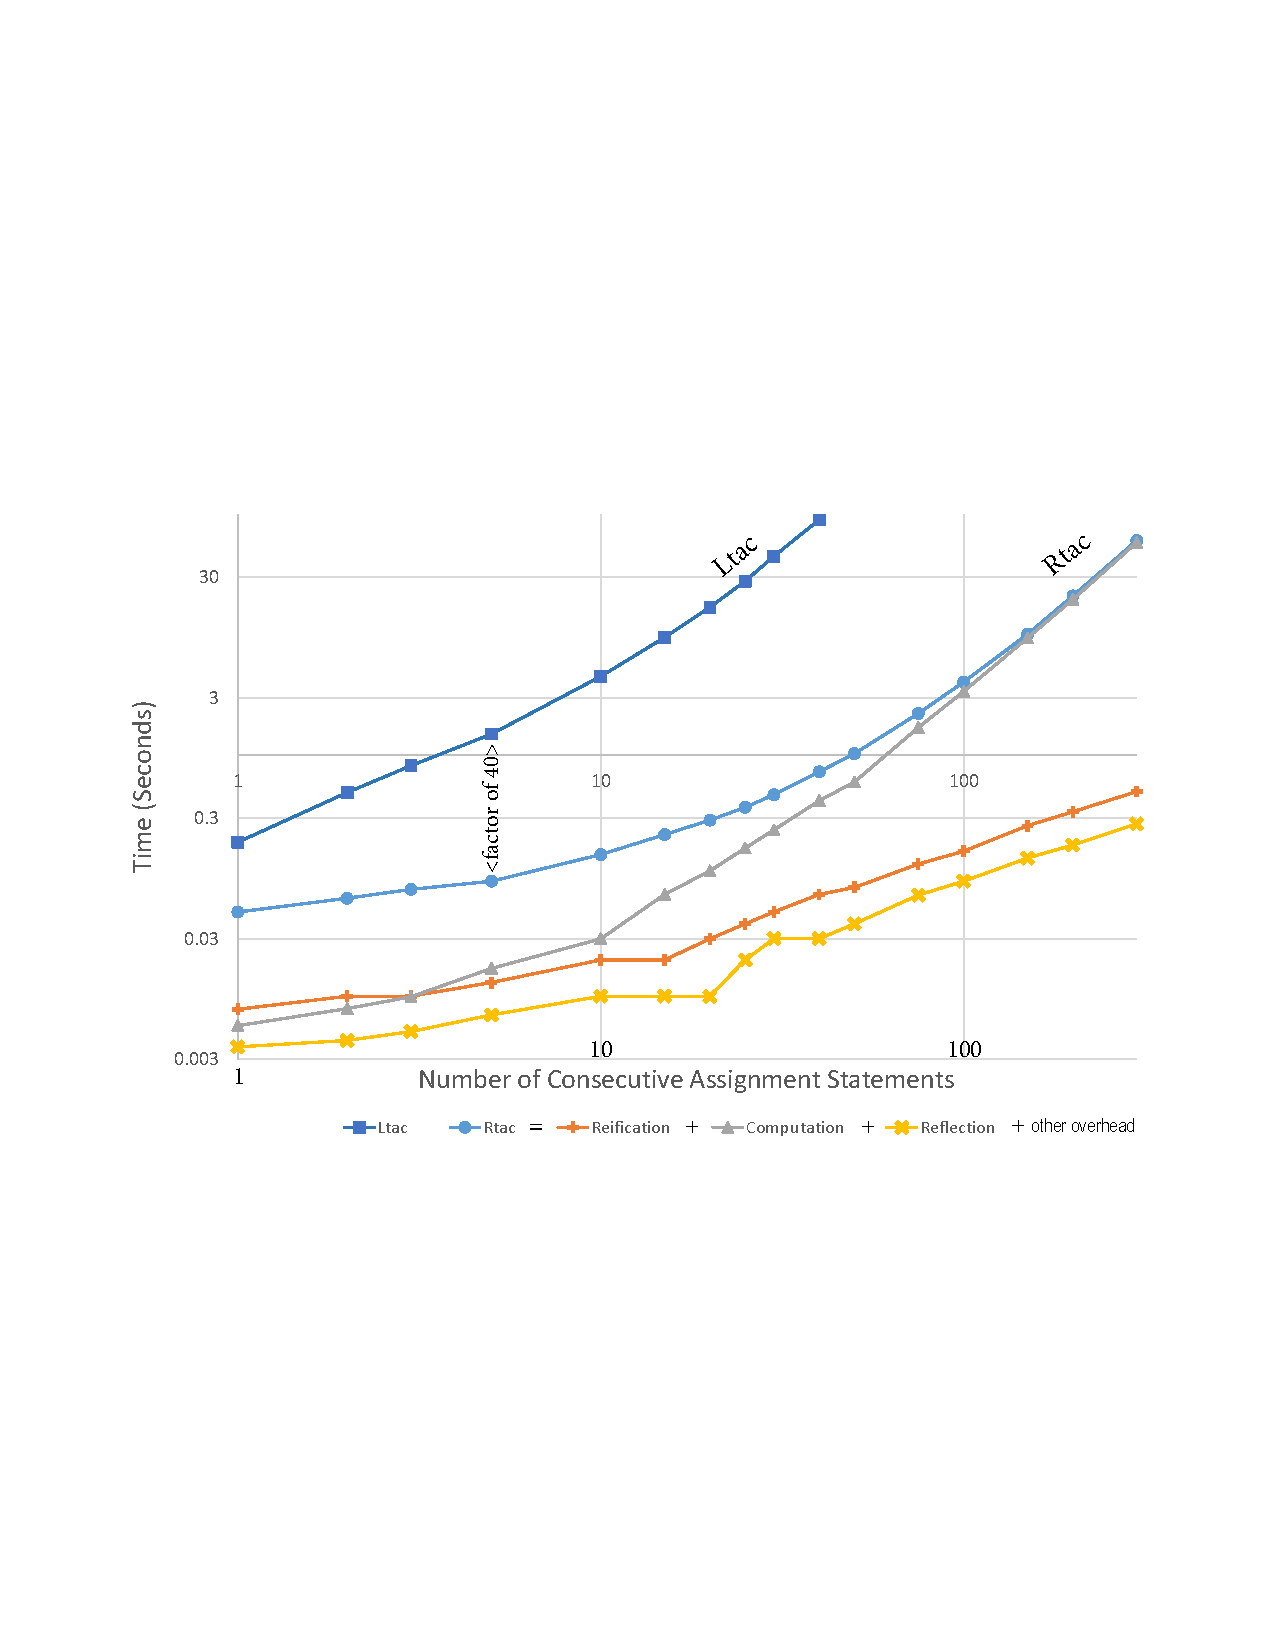
\includegraphics[width=\textwidth]{chart.pdf}
\vspace{-4ex}
\caption{Run time of Ltac vs Rtac, for $n$ consecutive C statements (log-log scale).}
\label{fig:chart}
\vspace{-4ex}
\end{figure}

Each data point is the average of 10 consecutive runs on a standard laptop. The
amount of memory on the laptop is over 2 gigabytes, which is the
maximum amount of memory that 32-bit Coq can use. Because it is very
difficult to get 64-bit Coq on all platforms, we attempt to write
tactics that can operate within the lower memory bounds.

Although this is a synthetic test, we consider
it a lower bound on the performance increase we will see in the
process of a real proof. This is because numerous other tests
indicate that for non-addressed variable assignments the size of the
precondition has the predominant effect on the run-time, not the
contents. This follows from what we would expect. The computation that
we need to do is almost all getting and setting from efficient tree
maps where get and set take $\log(n)$ time where $n$ is the largest
index that exists in the map. This is acceptable because we know that
our program input will be compiled by CompCert, and CompCert always
starts its variable indices with $1$, moving up sequentially. We can
be confident that this will always be the case because CompCert makes
use of PTrees. The remainder of the operations that RTac does are
linear (or slower) unifications between lemmas and proof goals, as
well as linear (or slower) rewrites by proved equalities. Repeated
linear operations are what lead to the polynomial operation we observe in
the chart above, not repeated $\log(n)$ gets and sets. 

The chart shows that there 
is a speedup of (typically) 40$\times$ (e.g., running $n\! = \! 8$ consecutive
C-program statements). 
Speedup improves with scale: $n\! =\! 50$ 
steps in Ltac takes over 2 minutes, while
the same number of steps in Rtac takes only .9 seconds, running almost 150$\times$ faster! 
Even for $n\!=\!1$ there is a 4$\times$ speedup.
This greatly improves interactivity of the logic. In general it
seems that growth of time relative to the number of program steps is
quadratic. Our benchmark that uses more complex preconditions
scales even better (not shown in a graph),
with 74$\times$ speedup at $n\! = \!10$.


The \emph{computation} curve, at the upper end, clearly
shows a time complexity of $n^{2.5}$.
This time complexity is roughly what we expect,
because (in this example) the
precondition grows linearly with the number of steps,
and each step has proof operations at least proportional to the size
of the precondition.



On a real-life example, a loop-body from 
OpenSSL's SHA function\footnote{The second loop body in
the \lstinline{sha256_block_data_order} function of the cited paper \cite{appel15:sha}; there are 850 nodes in the loop body's abstract synax tree.} 
takes 336 seconds to verify in our Ltac \lstinline{forward} tactic;
\lstinline|rforward| takes only 12 seconds---a 28$\times$ speedup. The sequence
includes 13 local-variable assignments,
5 loads, and 1 store, several of which contain 
huge mathematical expressions (resulting from macro-expansion in the
C source code). The assertions in that example
are large, with many local-variable and
spatial conjuncts.

Our computational theory of nested records yields 
a significant performance improvement.
Our \lstinline{data_at} benchmark verifies a sequence of 
4 loads and 4 stores
on a data structure represented by 8 spatial conjuncts,
taking 63 seconds in Ltac.  Using 
\lstinline{data_at}, with just one conjunct, 
verification takes 15 seconds in Ltac, a factor of 4 improvement.
We don't expect to see the same speedup in Rtac, which in
general is slower to be affected by changes in precondition size.

Unfortunately, after Rtac has efficiently computed a proof,
Coq's \lstinline|Qed| blows up, taking minutes  in some cases.
Qed blowups tend to occur when Coq cannot find an efficient
$\beta\eta$-conversion sequence to prove an equality
(even if the tactic script demonstrated one).
In the next section we discuss how to fix this.
Performance measurements in this section (for both Ltac and Rtac)
do not include Qed times; the Ltac Qed times are larger than
the Rtac Qed times, but both are terrible (e.g., 815 and 615 seconds,
respectively, for the SHA loop-body example).

While this is frustrating, as Coq continues to mature, even if Qed
time is slow, it won't cause too much frustration to the user. This is
because starting with Coq 8.5, proofs can be built and checked
asynchronously, allowing their statements to be used farther down in a
file while they build. A Qed time of a few minutes is inconsequential
as long as the user doesn't need to wait for it to continue proofs,
even proofs using the not-yet-checked proof. Furthermore, Coq 8.5 will allow for Coq .v
files to be compiled without checking proofs, making them very quickly
importable. Later it is possible to replace the unchecked object files
with object files. This means that libraries that are slow to build
can be built and usable rapidly, and then the actual work of checking
the proofs can be done in the background at the user's convenience.

\chapter{Conclusion}

\bibliographystyle{plain}
\bibliography{appel.bib}

\end{document}

